% Options for packages loaded elsewhere
\PassOptionsToPackage{unicode}{hyperref}
\PassOptionsToPackage{hyphens}{url}
%
\documentclass[
]{article}
\usepackage{amsmath,amssymb}
\usepackage{iftex}
\ifPDFTeX
  \usepackage[T1]{fontenc}
  \usepackage[utf8]{inputenc}
  \usepackage{textcomp} % provide euro and other symbols
\else % if luatex or xetex
  \usepackage{unicode-math} % this also loads fontspec
  \defaultfontfeatures{Scale=MatchLowercase}
  \defaultfontfeatures[\rmfamily]{Ligatures=TeX,Scale=1}
\fi
\usepackage{lmodern}
\ifPDFTeX\else
  % xetex/luatex font selection
\fi
% Use upquote if available, for straight quotes in verbatim environments
\IfFileExists{upquote.sty}{\usepackage{upquote}}{}
\IfFileExists{microtype.sty}{% use microtype if available
  \usepackage[]{microtype}
  \UseMicrotypeSet[protrusion]{basicmath} % disable protrusion for tt fonts
}{}
\makeatletter
\@ifundefined{KOMAClassName}{% if non-KOMA class
  \IfFileExists{parskip.sty}{%
    \usepackage{parskip}
  }{% else
    \setlength{\parindent}{0pt}
    \setlength{\parskip}{6pt plus 2pt minus 1pt}}
}{% if KOMA class
  \KOMAoptions{parskip=half}}
\makeatother
\usepackage{xcolor}
\usepackage[margin=1in]{geometry}
\usepackage{color}
\usepackage{fancyvrb}
\newcommand{\VerbBar}{|}
\newcommand{\VERB}{\Verb[commandchars=\\\{\}]}
\DefineVerbatimEnvironment{Highlighting}{Verbatim}{commandchars=\\\{\}}
% Add ',fontsize=\small' for more characters per line
\usepackage{framed}
\definecolor{shadecolor}{RGB}{248,248,248}
\newenvironment{Shaded}{\begin{snugshade}}{\end{snugshade}}
\newcommand{\AlertTok}[1]{\textcolor[rgb]{0.94,0.16,0.16}{#1}}
\newcommand{\AnnotationTok}[1]{\textcolor[rgb]{0.56,0.35,0.01}{\textbf{\textit{#1}}}}
\newcommand{\AttributeTok}[1]{\textcolor[rgb]{0.13,0.29,0.53}{#1}}
\newcommand{\BaseNTok}[1]{\textcolor[rgb]{0.00,0.00,0.81}{#1}}
\newcommand{\BuiltInTok}[1]{#1}
\newcommand{\CharTok}[1]{\textcolor[rgb]{0.31,0.60,0.02}{#1}}
\newcommand{\CommentTok}[1]{\textcolor[rgb]{0.56,0.35,0.01}{\textit{#1}}}
\newcommand{\CommentVarTok}[1]{\textcolor[rgb]{0.56,0.35,0.01}{\textbf{\textit{#1}}}}
\newcommand{\ConstantTok}[1]{\textcolor[rgb]{0.56,0.35,0.01}{#1}}
\newcommand{\ControlFlowTok}[1]{\textcolor[rgb]{0.13,0.29,0.53}{\textbf{#1}}}
\newcommand{\DataTypeTok}[1]{\textcolor[rgb]{0.13,0.29,0.53}{#1}}
\newcommand{\DecValTok}[1]{\textcolor[rgb]{0.00,0.00,0.81}{#1}}
\newcommand{\DocumentationTok}[1]{\textcolor[rgb]{0.56,0.35,0.01}{\textbf{\textit{#1}}}}
\newcommand{\ErrorTok}[1]{\textcolor[rgb]{0.64,0.00,0.00}{\textbf{#1}}}
\newcommand{\ExtensionTok}[1]{#1}
\newcommand{\FloatTok}[1]{\textcolor[rgb]{0.00,0.00,0.81}{#1}}
\newcommand{\FunctionTok}[1]{\textcolor[rgb]{0.13,0.29,0.53}{\textbf{#1}}}
\newcommand{\ImportTok}[1]{#1}
\newcommand{\InformationTok}[1]{\textcolor[rgb]{0.56,0.35,0.01}{\textbf{\textit{#1}}}}
\newcommand{\KeywordTok}[1]{\textcolor[rgb]{0.13,0.29,0.53}{\textbf{#1}}}
\newcommand{\NormalTok}[1]{#1}
\newcommand{\OperatorTok}[1]{\textcolor[rgb]{0.81,0.36,0.00}{\textbf{#1}}}
\newcommand{\OtherTok}[1]{\textcolor[rgb]{0.56,0.35,0.01}{#1}}
\newcommand{\PreprocessorTok}[1]{\textcolor[rgb]{0.56,0.35,0.01}{\textit{#1}}}
\newcommand{\RegionMarkerTok}[1]{#1}
\newcommand{\SpecialCharTok}[1]{\textcolor[rgb]{0.81,0.36,0.00}{\textbf{#1}}}
\newcommand{\SpecialStringTok}[1]{\textcolor[rgb]{0.31,0.60,0.02}{#1}}
\newcommand{\StringTok}[1]{\textcolor[rgb]{0.31,0.60,0.02}{#1}}
\newcommand{\VariableTok}[1]{\textcolor[rgb]{0.00,0.00,0.00}{#1}}
\newcommand{\VerbatimStringTok}[1]{\textcolor[rgb]{0.31,0.60,0.02}{#1}}
\newcommand{\WarningTok}[1]{\textcolor[rgb]{0.56,0.35,0.01}{\textbf{\textit{#1}}}}
\usepackage{longtable,booktabs,array}
\usepackage{calc} % for calculating minipage widths
% Correct order of tables after \paragraph or \subparagraph
\usepackage{etoolbox}
\makeatletter
\patchcmd\longtable{\par}{\if@noskipsec\mbox{}\fi\par}{}{}
\makeatother
% Allow footnotes in longtable head/foot
\IfFileExists{footnotehyper.sty}{\usepackage{footnotehyper}}{\usepackage{footnote}}
\makesavenoteenv{longtable}
\usepackage{graphicx}
\makeatletter
\def\maxwidth{\ifdim\Gin@nat@width>\linewidth\linewidth\else\Gin@nat@width\fi}
\def\maxheight{\ifdim\Gin@nat@height>\textheight\textheight\else\Gin@nat@height\fi}
\makeatother
% Scale images if necessary, so that they will not overflow the page
% margins by default, and it is still possible to overwrite the defaults
% using explicit options in \includegraphics[width, height, ...]{}
\setkeys{Gin}{width=\maxwidth,height=\maxheight,keepaspectratio}
% Set default figure placement to htbp
\makeatletter
\def\fps@figure{htbp}
\makeatother
\setlength{\emergencystretch}{3em} % prevent overfull lines
\providecommand{\tightlist}{%
  \setlength{\itemsep}{0pt}\setlength{\parskip}{0pt}}
\setcounter{secnumdepth}{-\maxdimen} % remove section numbering
\renewcommand{\figurename}{Figura}
\renewcommand{\tablename}{Tabla}
\usepackage{float}
\floatplacement{figure}{H}
\usepackage{titling}
\usepackage{lipsum}
\usepackage{fancyhdr}
\usepackage{etoolbox}
\usepackage{setspace}
\usepackage{titlesec}
\usepackage{emptypage}
\pagestyle{fancy}
\usepackage{placeins}
\fancyhf{}
\patchcmd{\maketitle}{\@maketitle}{\centering\vspace*{4cm}\@maketitle}{}{}
\thispagestyle{empty}
\ifLuaTeX
  \usepackage{selnolig}  % disable illegal ligatures
\fi
\usepackage{bookmark}
\IfFileExists{xurl.sty}{\usepackage{xurl}}{} % add URL line breaks if available
\urlstyle{same}
\hypersetup{
  hidelinks,
  pdfcreator={LaTeX via pandoc}}

\author{}
\date{\vspace{-2.5em}}

\begin{document}

\begin{titlepage}
\centering
\vspace*{4cm} % espacio superior

{\Huge \textbf{Trabajo práctico 1 Estadística Bayesiana}}\\[2cm]

{\Large Agustina Roura}\\[0.5cm]
{\Large Cristian Nahuel Coveñas}\\[0.5cm]
{\Large Juan Sebastian Reines}\\[2cm]

{\large Fecha: Abril 2025}

\vfill

\end{titlepage}

\newpage

\subsection{Introducción}\label{introducciuxf3n}

Las apuestas en línea han ganado una creciente popularidad entre los adolescentes, impulsadas por la accesibilidad de plataformas digitales y la constante exposición a la publicidad en redes sociales y eventos deportivos. En principio, creen tener el ``control'', pero la realidad resulta ser mucho más compleja: quedan atrapados en una nube de rachas ganadoras y, cuando comienzan a perder dinero, continúan apostando con la esperanza de recuperarlo.

Además de esto el poder realizar estudios sobre el tema es complejo, a muchos adolescentes les causa vergüenza el admitir que practican dichas apuestas, por lo que optan por no responder con sinceridad a ciertas preguntas, por ejemplo en el marco de una encuesta. Este fenómeno, conocido como sesgo de respuesta, representa un desafío para quienes buscan obtener datos fiables en encuestas y estudios sobre este tema.

Partiendo de la premisa de que una forma de incrementar la cooperación de los encuestados es garantizar la protección de información sensible, una posible forma de mitigar este sesgo es la técnica de respuesta aleatorizada, que permite que los encuestados respondan de manera más sincera sin temor a ser identificados. En la técnica de respuesta aleatorizada, se introduce una cuota de azar con el objetivo de preservar la privacidad de la persona que responde.

Estudiaremos dos técnicas de respuesta aleatorizada y nos centraremos en el problema de querer realizar inferencias sobre \(\pi_a\), la proporción de estudiantes de una escuela que participan de apuestas deportivas en línea.

\newpage

\subsection{Índice}\label{uxedndice}

1.\hyperref[Objetivo-1]{\textbf{El efecto de la mentira en las estimaciones}}

2.\hyperref[Objetivo-2]{\textbf{Método de Warner}}

3.\hyperref[Objetivo-3]{\textbf{Método de Greenberg}}

4.\hyperref[Objetivo-4]{\textbf{Comparación entre los métodos y los niveles de mentira}}

\newpage

\subsection{El efecto de la mentira en las estimaciones}\label{Objetivo-1}

Dado que el tema de las apuestas en línea puede resultar delicado para muchos estudiantes, se considera que varios de ellos podrían optar por no responder con total sinceridad a la encuesta realizada. Esta posible falta de veracidad introduce un sesgo en los datos recolectados, lo que justifica la necesidad de un enfoque estadístico que permita incorporar dicha incertidumbre en el análisis.

Con este objetivo, se propone un modelo bayesiano centrado en el parámetro de interés, denotado como \(\pi_a\), que representa la proporción real de estudiantes que apuestan en línea. Este enfoque considera diferentes grados de falta de sinceridad en las respuestas, introduciendo un nuevo parámetro (conocido), \(\mu\), que corresponde a la probabilidad de que un estudiante que apuesta mienta al responder.

Con el fin de realizar estudios comparativos, se asumirá que en la población el porcentaje de estudiantes que han participado en apuestas en línea es del 40\%. A partir de esta suposición, se simularán muestras de tamaño n = 100, considerando que los estudiantes que efectivamente han apostado alguna vez pueden mentir al responder, con una probabilidad denotada por \(\mu\).

\subsubsection{Modelo bayesiano Beta-Binomial}\label{subtitulo-1}

\begin{itemize}
\item
  \(\pi_a\): Proporción de estudiantes de una escuela que participan de apuestas deportivas en línea.
\item
  \(n\): Cantidad de estudiantes encuestados.
\item
  \(y\): Número de estudiantes que apuestan.
\end{itemize}

\paragraph{Prior:}\label{prior}

Considerando la naturaleza del parámetro, se busca asignar una credibilidad a priori a los posibles valores de \(\pi_a\). Esta credibilidad puede modelarse mediante una distribución beta, con el objetivo de reflejar que todos los valores entre 0 y 1 son igualmente probables. En particular, se utilizo una distribución uniforme, es decir, una distribución beta con parámetros \(a\) = 1 y \(b\) = 1.
\[ \pi_a \sim Beta(a = 1, b = 1) \]

\FloatBarrier

\paragraph{Likelihood:}\label{likelihood}

El \(likelihood\) es una función que mide cuán probable es observar los datos \(y_i\) dado un valor especifico del parámetro \(\pi_a\), es decir, evalúa la probabilidad de los datos en función del parámetro.
\[ y \mid \pi_a \sim Bin(n , \pi_a) \]

\FloatBarrier

\paragraph{Posterior:}\label{posterior}

La distribución a posteriori representa nuestro conocimiento actualizado sobre un parámetro después de haber observado los datos. Se obtiene como el producto entre el \(prior\) (lo que se creía antes) y el \(likelihood\) (la verosimilitud de los datos).
\[ p(\pi_a/y) \propto p(y/\pi_a).p(\pi_a) \]

\begin{figure}
\centering
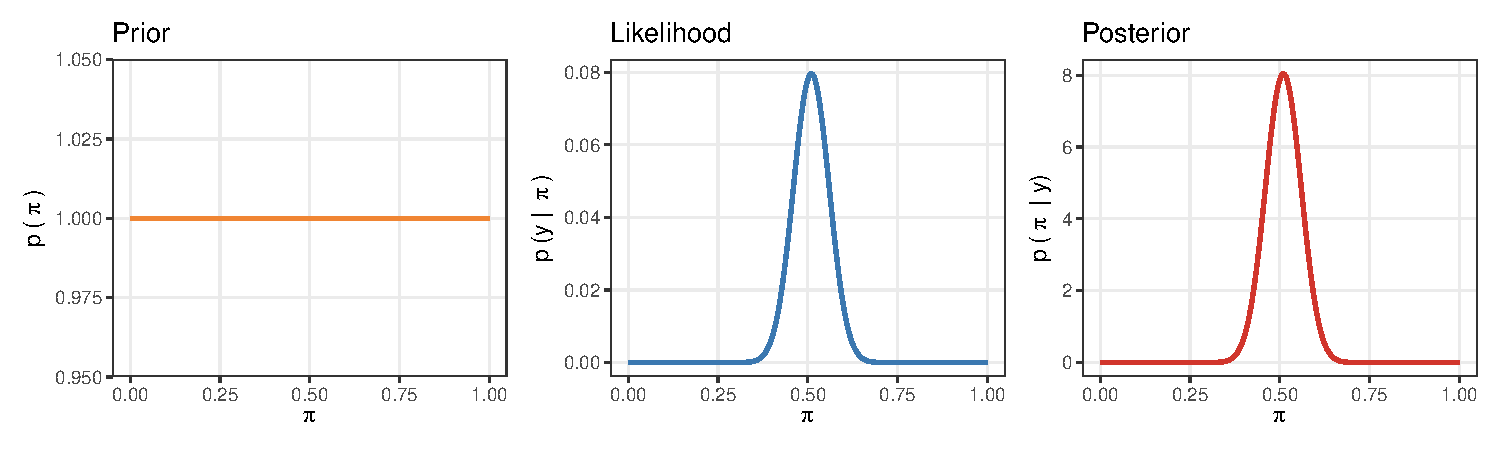
\includegraphics{TP-1--Bayes_files/figure-latex/fig1-1.pdf}
\caption{\label{fig:fig1}Distribución del modelo bayesiano}
\end{figure}

Partiendo de una creencia inicial en la que todos los valores posibles de \(\pi_a\) son igualmente probables, se observa en la Figura \ref{fig:fig1} que la verosimilitud (\(likelihood\)) y el \(posterior\) son similares. Esto se debe a que la elección del \(prior\) no afecta directamente al \(posterior\), lo que genera que tenga una forma distribucional similar a la de la verosimilitud de los datos.

\subsubsection{Niveles de mentira de los estudiantes}\label{subtitulo-2}

Si se toma en cuenta de que hay una probabilidad de que los estudiantes
mientan, se simularon muestras de estudiantes con distintos niveles de
mentira bajo, medio y alto; para poder ver el comportamiento de la
variable de interés con cada nivel de mentira

\FloatBarrier

\begin{figure}

{\centering 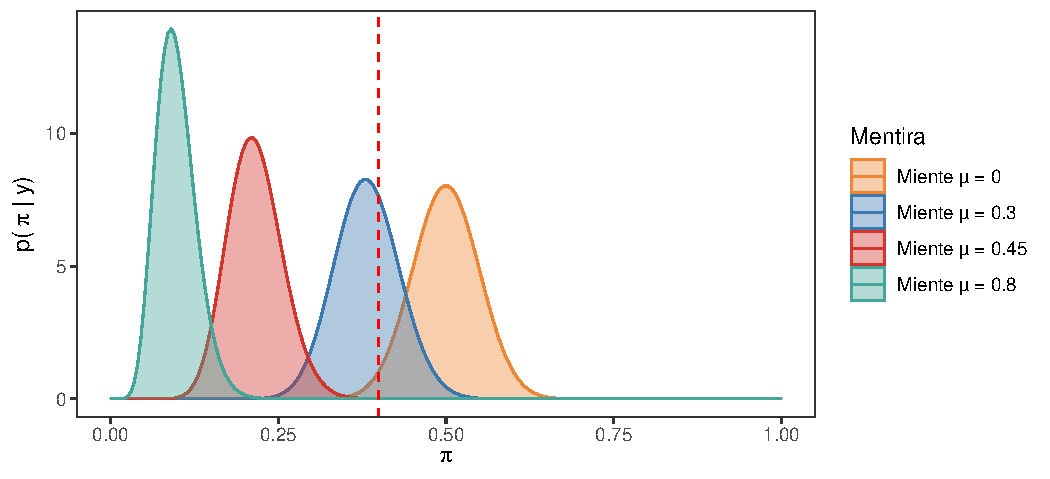
\includegraphics{TP-1--Bayes_files/figure-latex/fig2-1} 

}

\caption{Posterior para diferentes niveles de mentira}\label{fig:fig2}
\end{figure}

De la Figura \ref{fig:fig2} se puede ver como a medida que aumenta la probabilidad de que un estudiante mienta, se observó que la variabilidad del \(posterior\) es cada vez más chica, pero tiende a centrarse en un valor sesgado distinto al del parámetro de interés \(\pi_a\).

\newpage

\subsubsection{Aumento de la cantidad de simulaciones}\label{subtitulo-3}

Para interpretar mejor los resultados de la inferencia, se recurre a las simulaciones de 1000 muestras del \(posterior\) para cada nivel de mentira \(\mu\), con el interés de estimar los intervalos de credibilidad, los cuales buscan determinar qué cantidad de los intervalos del 90\% para cada posterior contiene al verdadero parámetro \(\pi_a\).

\begin{figure}

{\centering 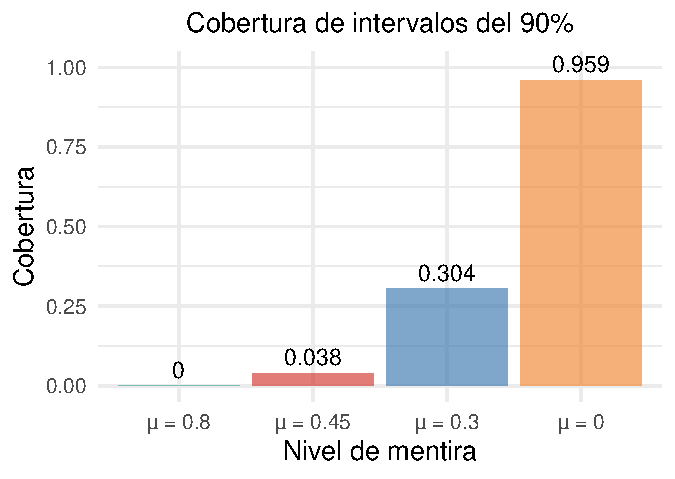
\includegraphics{TP-1--Bayes_files/figure-latex/fig3-1} 

}

\caption{Comparación entre los niveles de mentira}\label{fig:fig3}
\end{figure}

Como se observa en la Figura \ref{fig:fig3}, en las muestras generadas a partir de una población donde el nivel de \(\mu\) es nulo, la cobertura de los intervalos de credibilidad para el verdadero valor del parámetro es superior en comparación con los niveles más altos de \(\mu\). Por lo tanto, el supuesto de no mentira es influyente en las inferencias realizadas sobre el parámetro \(\pi_a\) para las distintas técnicas de respuesta aleatorizada.

\clearpage

\subsection{Método de Warner}\label{Objetivo-2}

Este es un método de aleatorización, en el cual se le hace la pregunta a
el estudiante con probabilidad \(p\) ``¿Alguna vez participaste de apuestas
deportivas?'' y con probabilidad \((1 - p)\) ``¿Nunca ha participado en
apuestas deportivas?''

Esta estrategia permite preservar la privacidad del encuentado y obtener
una estimación de \(\pi_a\).

\subsubsection{Respuesta del estudiante}\label{subtitulo-4}

A continuación se utilizó el método de Warner para calcular la probabilidad de que un estudiante responda afirmativamente, cualquiera sea la pregunta y tambien la probabilidad de que un estudiante responda negativamente, cualquiera sea la pregunta.

\begin{itemize}
\item
  \(y^* : \text{El estudiante responde afirmativamente. } P(y^*) = \lambda_W\)
\item
  \(\lambda_W :\) Probabilidad de que un estudiante responda
  afirmativamente
\item
  \(1 - \lambda_W :\) Probabilidad de que un estudiante no responda
  afirmativamente
\item
  \(Q : \text{Pregunta 1 (¿participas en apuestas en linea?). } P(Q)=p \ conocido\)
\item
  \(Q^c : \text{Pregunta 2 (¿no participas en apuestas en linea?). } P(Q^c)=(1-p) \ conocido\)
\end{itemize}

Para la probabilidad de que un estudiante responda afirmativamente,
tomamos el método de probabilidad total
\[ \lambda_W = P(y^*) = P(y^*,Q) + P(y^*,Q^c)\]
\[\\ = P(y^* \mid Q) \cdot P(Q) + P(y^* \mid Q^c) \cdot P(Q^c) \]
\[\\= \pi_a \cdot p + (1 - \pi_a) \cdot (1 - p)\]

Para la probabilidad de que un estudiante responda de forma negativa
\[ 1 - \lambda_W = P(y^{*c}) = P(y^{*c},Q) + P(y^{*c},Q^c)\]
\[\\ = P(y^{*c} \mid Q) \cdot P(Q) + P(y^{*c} \mid Q^c) \cdot P(Q^c) \]
\[\\= (1 - \pi_a) \cdot p + \pi_a \cdot (1 - p)\]

\subsubsection{Modelo razonable}\label{subtitulo-5}

En base al análisis realizado anteriormente de se planteó el siguiente modelo para la generación de los datos.

\begin{itemize}
\item
  \(y^*\): El estudiante responde afirmativamente
\item
  \(\pi_a\): Proporción de estudiantes que apuestan
\end{itemize}

\[\text{Prior}\] \[\pi_a \ \sim \ Beta(a = 1, b = 1)\]
\[\text{Likelihood}\]
\[y^* \text{| }\pi_a \sim \text{Bin}(n,\lambda_W), \text{ con } \lambda_W \text{ función de } \pi_a\]

\subsubsection{Planteo a partir de un Prior con distribución Uniforme}\label{subtitulo-6}

Se realiza todo el procedimiento matemático correspondiente para la utilización de un \(prior\) con una distribución uniforme para llegar a un \(posterior\) exacto

\[\pi_a \sim \text{Beta}(1,1)\]
\[y^* \mid \pi_a \sim \text{Bin}(n, \lambda_W),\text{ con } \lambda_W \text{ función de } \pi_a\\\]
\[P(\pi_a \mid y^*) = \dfrac{P(y^* \mid \pi_a) \cdot P(\pi_a)}{\int_{0}^{1} P(y^* \mid \pi_a)d\pi_a} \quad \text{Por regla de Bayes}\]
\[P(\pi_a \mid y^*) =  \dfrac{\binom{N}{y^*} \lambda^{y^*} (1 - \lambda)^{N - y^*}}{\int_{0}^{1} \binom{N}{y^*} \lambda^{y^*} (1 - \lambda)^{N - y^*} \, d\pi_a}\\\]
\[P(\pi_a \mid y^*) =  \dfrac{ \lambda^{y^*} (1 - \lambda)^{N - y^*}}{\int_{0}^{1} \lambda^{y^*} (1 - \lambda)^{N - y^*} \, d\pi_a}\\\]

\[P(\pi_a \mid y^*) = \dfrac{\lambda^{y^*} (1 - \lambda)^{N - y^*}}{Z}\\\]
\[\text{Donde }\lambda \text{ = } \pi_a p + (1 - \pi_a)(1 - p) \text{, podemos reemplazar}\]
\[P(\pi_a \mid y^*) = \dfrac{[\pi_a p + (1 - \pi_a)(1 - p)]^{y^*} [(1 - \pi_a)p + (1 - \pi_a)(1 - p)]^{N - y^*}}{Z}\\\]

\[\text{Donde se tiene que Z = } \int_{0}^{1} [\pi_a p + (1 - \pi_a)(1 - p)]^{y^*} [(1 - \pi_a)p + (1 - \pi_a)(1 - p)]^{N - y^*} d\pi_a\]
\[\text{Aplicando sustitución:}\]
\[\lambda = \pi_a p + (1 - \pi_a)(1 - p) \]
\[  d\lambda = 2p \ - \ 1 \ d\pi_a \implies d\pi_a = \dfrac{d\lambda}{2p-1}\]
\[\text{Cuando }\pi_a = 0, \text{ luego } \lambda = (1-p) \text{ y cuando }\pi_a =1, \text{ luego } \lambda= p\]
\[\text{Quedando Z = } \int_{1-p}^{p} \lambda^{y^*} (1 - \lambda)^{N - y^*} \dfrac{ d\lambda}{2p -1}\]
\[\text{Z = } \dfrac{1}{2p -1} \left[\int_{0}^{p} \lambda^{(y^*+1)-1} (1 - \lambda)^{(N - y^*+1)-1} d\lambda - \int_{0}^{1-p} \lambda^{(y^*+1)-1} (1 - \lambda)^{(N - y^*+1)-1} d\lambda\right]\]
\[\text{Sabiendo que B(}x,\ a,\ b)\ = \int_{0}^{x} t^{a-1}(1 - t)^{b-1} dt \text{, es la función beta incompleta se tiene que:}\]
\[Z = \dfrac{B(p,\ y^*+1,\ N-y^* +1)\ -\ B(1-p,\ y^*+1,\ N-y^* +1)}{2p-1}\]

\newpage

\subsubsection{Visualización de Posterior}\label{subtitulo-7}

Para sumar al análisis se realizaron gráficos de los \(posterior\) utilizando
distintos valores de \(p\), por lo que se simularon distintas muestras para
poder ver el comportamiento en cada \(p\) propuesto

\begin{figure}

{\centering 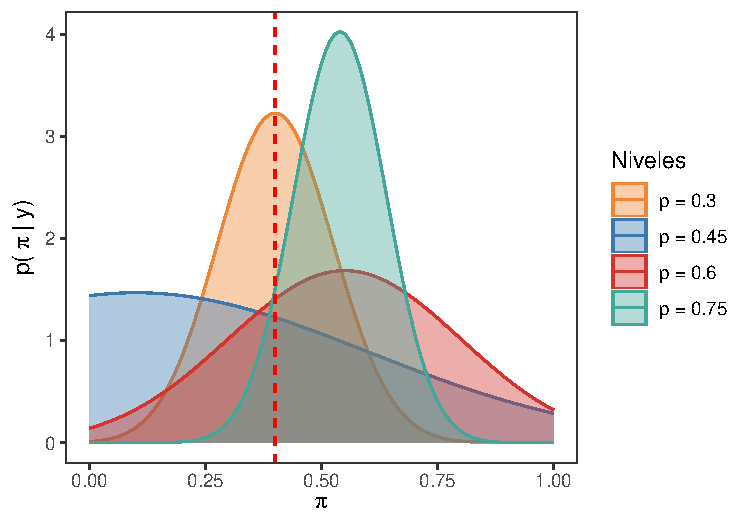
\includegraphics{TP-1--Bayes_files/figure-latex/fig4-1} 

}

\caption{Posterior para distintos valores de p}\label{fig:fig4}
\end{figure}

A partir de la simulación del método de Warner utilizando distintos valores de \(p\), se observó en la Figura \ref{fig:fig4} que el comportamiento de las distribuciones a posteriori varía notablemente según el nivel de \(p\) utilizado. En particular, cuando se utilizan valores extremos de \(p\), como \(p = 0.3\) y \(p = 0.4\), las distribuciones a posteriori tiende a concentrarse en torno al verdadero valor de \(\pi_a\), presentando menor variabilidad. Esto indica que, en estos casos, la información proporcionada por la muestra es más determinante para actualizar la creencia sobre el parámetro de interés.

Por otro lado, para los valores de \(p\) más centrales, como \(p = 0.45\) o \(p = 0.6\), las distribuciones resultan más dispersas, reflejando una mayor incertidumbre en la estimación de \(\pi_a\). En resumen, el valor de \(p\) influye directamente en la precisión de la distribución a posteriori, por lo que debe ser cuidadosamente considerado al momento de implementar este tipo de técnicas en estudios empíricos. Además de la influencia del valor de \(p\), también se debe considerar el rol que juega la aleatoriedad de las muestras obtenidas.

\newpage

\subsubsection{¿Y si la población cambia?}\label{subtitulo-8}

Lo que es un aspecto crucial a considerar, hasta este punto, el análisis se ha desarrollado bajo el supuesto de una población con un valor de \(\pi_a\) definido. Sin embargo, la modificación de este valor de \(\pi_a\) sin duda influirá en nuestras inferencias y, por ende, en las conclusiones.

\begin{center}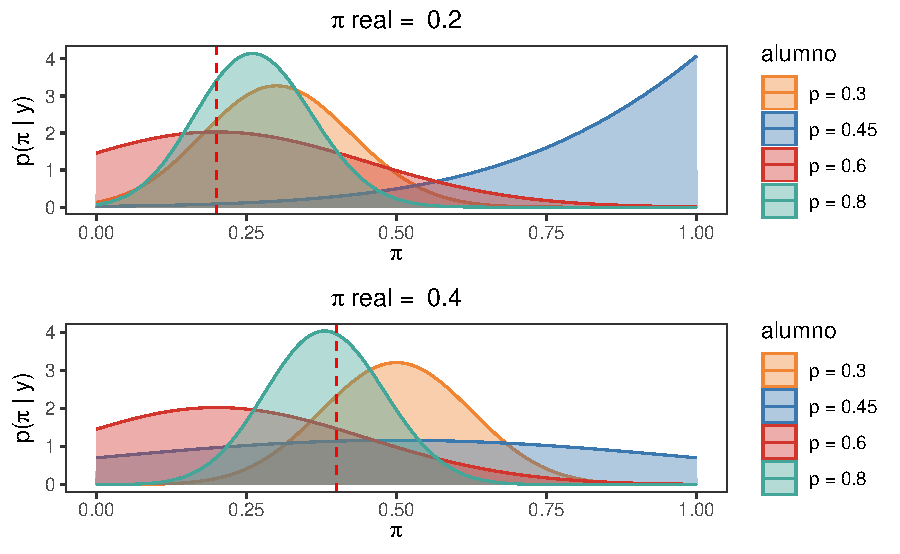
\includegraphics{TP-1--Bayes_files/figure-latex/unnamed-chunk-6-1} \end{center}
\begin{figure}

{\centering 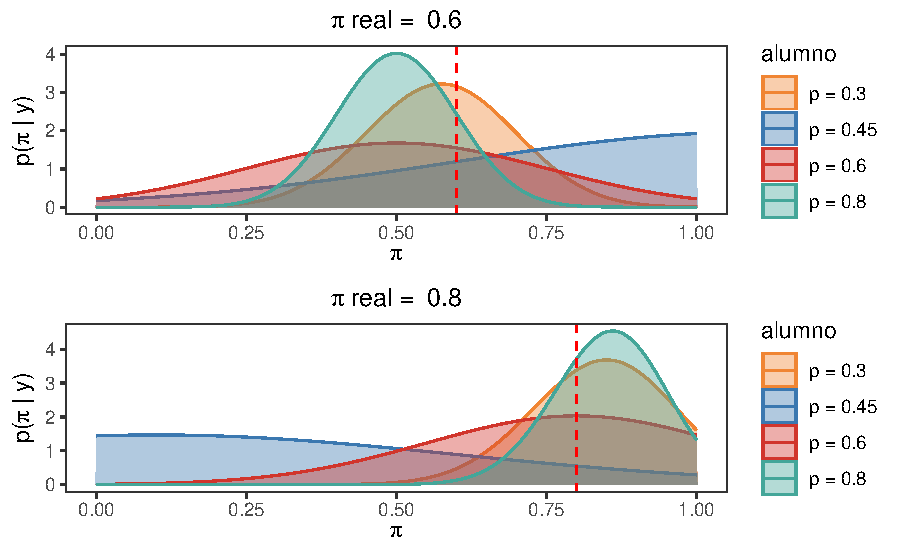
\includegraphics{TP-1--Bayes_files/figure-latex/fig5-1} 

}

\caption{Posterior segun distintas poblaciones}\label{fig:fig5}
\end{figure}

Como se observa en la Figura \ref{fig:fig5} a pesar de que las poblaciones son distintas, se puede ver como para la mayoria de graficos en general el comportamiento más variable es cuando \(p = 0.45\) lo cual nos ayuda a entender que si el \(p\) es cercano a 0.5 menos información de la realidad nos puede aportar cada muestra aumentando la variabilidad de la incertidumbre para el parámetro de interés \(\pi_a\)

A medida que aumenta la cantidad de estudaintes que apuestan en la poblacion se observa que para los diferentes \(p\) la variabilidad gira en torno al verdadero valor de \(\pi_a\) para los casos más extremos, \(p = 0.3\) y \(p = 0.8\). Mientras que para los casos de \(p = 0.45\) y \(p = 0.6\) se nota una mayor variabilidad entre las poblaciones como son muy variables no podemos obtener una buena precisión al verdadero valor.

Cuando el valor de \(p\) es más cercano a 0.5 el método Warner presenta una gran incertidumbre respecto a cuál es la pregunta realizada a cada persona, lo que dificulta el discernimiento de quiénes realmente participan de la actividad sensible. En cambio cuando el valor de p se aleja de 0.5, en particular hacia los extremos, esta ambigüedad en las respuestas disminuye, lo que otorga una mayor claridad a la hora de interpretar los resultados respecto a la proporción de personas que realizan apuestas online.

\subsubsection{Recursos para proximos análisis}\label{subtitulo-9}

Se consideró la opción de realizar una función que permita extender los resultados del análisis realizado. De modo de poder replicar este estudio y sus inferencias de forma aproximada, pudiendo considerar un prior con una distribución diferente a la beta(1,1).

\begin{Shaded}
\begin{Highlighting}[]
\CommentTok{\#función del posterior para un prior no necesariamente uniforme}

\NormalTok{posterior\_war }\OtherTok{\textless{}{-}} \ControlFlowTok{function}\NormalTok{(pi, p, a, b)\{}
  \CommentTok{\# Establecemos la función lambda del método warner}
\NormalTok{  lambda\_W }\OtherTok{\textless{}{-}} \ControlFlowTok{function}\NormalTok{(p, pi\_a)\{}\FunctionTok{return}\NormalTok{(pi\_a}\SpecialCharTok{*}\NormalTok{p }\SpecialCharTok{+}\NormalTok{ (}\DecValTok{1}\SpecialCharTok{{-}}\NormalTok{p)}\SpecialCharTok{*}\NormalTok{(}\DecValTok{1}\SpecialCharTok{{-}}\NormalTok{pi\_a))\}}
  \CommentTok{\# Simulamos una muestra de respuestas afirmativas con el parametro lambda\_w}
\NormalTok{  y }\OtherTok{\textless{}{-}} \FunctionTok{rbinom}\NormalTok{(}\DecValTok{1}\NormalTok{,}\DecValTok{100}\NormalTok{,}\FunctionTok{lambda}\NormalTok{(p, pi))}
  \CommentTok{\# Construimos el numerador del posterior aproximado}
\NormalTok{  num }\OtherTok{\textless{}{-}} \FunctionTok{dbeta}\NormalTok{(pi\_grid, a, b) }\SpecialCharTok{*} \FunctionTok{dbinom}\NormalTok{(y, }\DecValTok{100}\NormalTok{, }\FunctionTok{lambda}\NormalTok{(p, pi\_grid))}
  \CommentTok{\# Construimos el denominador del posterior aproximado}
\NormalTok{  delta }\OtherTok{\textless{}{-}} \FunctionTok{diff}\NormalTok{(pi\_grid)[}\DecValTok{1}\NormalTok{] }
\NormalTok{  denom }\OtherTok{\textless{}{-}} \FunctionTok{sum}\NormalTok{(num) }\SpecialCharTok{*}\NormalTok{ delta}
  \CommentTok{\# Obtenemos el Posterior aproximado}
\NormalTok{  posterior }\OtherTok{\textless{}{-}}\NormalTok{ num }\SpecialCharTok{/}\NormalTok{ denom}
  \FunctionTok{return}\NormalTok{(posterior)}
\NormalTok{\}}
\end{Highlighting}
\end{Shaded}

\newpage

\subsection{Método Greenberg}\label{Objetivo-3}

\subsubsection{Probabilidad de respuesta afirmativa segun el método Greenberg}\label{subtitulo-10}

Esta técnica de respuesta aleatoria consiste en presentar una de dos
posibles preguntas al alumno encuestado, con probabilidad \(p\), se le
pregunta sobre el tema de interés (¿Realiza apuestas deportivas en
linea?), y con probabilidad \(1-p\), se le pregunta sobre un tema no
relacionado del cual se conoce la probabilidad a priori (¿Naciste en un
mes con 31 días?)

Esta estrategia permite preservar la privacidad del encuentado y obtener
una estimación de \(\pi_a\). Se asume que se conoce de antemano la
proporción de personas que pertenecen a la categoria B no relacionado al tema de interes
(\(\pi_B = \dfrac{7}{12}\))

En el marco del método propuesto por Greenberg, es de interés conocer la
probabilidad de que un individuo responda afirmativamente o
negativamente a la pregunta que se le presenta. Dado que la técnica
implica un mecanismo aleatorio donde las personas pueden ser consultadas
sobre una categoría sensible o una no sensible con determinadas
probabilidades, la respuesta observada no refleja directamente la
verdadera pertenencia del individuo a una categoría, sino una
combinación probabilística de ambas posibilidades.

\begin{itemize}
\item
  \(y^* \text{ : } \text{El estudiante responde afirmativamente } P(y^*) = \lambda_G\)
\item
  \(\lambda_G\) : Probabilidad de que un estudiante responda
  afirmativamente
\item
  \(1 - \lambda_G\) : Probabilidad de que un estudiante no responda
  afirmativamente
\item
  \(\pi_a\) : Probabilidad de que un estudiante realice apuestas online
\item
  \(\pi_B \text{ : } \text{Probabilidad de que un estudiante pertenezca a la categoria B. } P(\pi_b) = \dfrac{7}{12}\)
\item
  \(Q_1 \text{ : } \text{Pregunta 1 (¿Participas en apuestas en linea?). } P(Q)=p \ conocido\)
\item
  \(Q_2 \text{ : } \text{Pregunta 2 (¿Es cierto que naciste en un mes con 31 dias?). } P(Q_2)=(1-p) \ conocido\)
\end{itemize}

Para la probabilidad de que un estudiante responda afirmativamente,
tomamos el método de probabilidad total

\[ \lambda_G = P(y^*) = P(y^*,Q_1) + P(y^*,Q_2)\]
\[\\ = P(y^* \mid Q_1) \cdot P(Q_1) + P(y^* \mid Q_2) \cdot P(Q_2) \]
\[\\= \pi_a \cdot p + \pi_B \cdot (1 - p)\]
\[\\= \pi_a \cdot p + \dfrac{7}{12} \cdot (1 - p)\]

Para la probabilidad de que un estudiante responda de forma negativa

\[ P(y^{*c}) = P(y^{*c},Q_1) + P(y^{*c},Q_2)\]
\[\\= P(y^{*c} \mid Q_1) \cdot P(Q_1) + P(y^{*c} \mid Q_2) \cdot P(Q_2)\]
\[\\= (1 - \pi_a) \cdot p + (1 - \pi_B) \cdot (1 - p)\]
\[\\= (1 - \pi_a) \cdot p + \dfrac{5}{12} \cdot (1 - p)\]

Estos valores permiten establecer el vínculo entre las respuestas
observadas y la proporción real de interés en la población.

\[\text{Prior}\] \[ \pi_a \sim Beta(a = 1, b = 1) \\\]
\[\text{Likelihood}\]
\[y^*\text{| }\pi_a \sim \text{Bin}(n, \lambda_G), \text{ con } \lambda_G \text{ función de } \pi_a \\\]

Una vez conocida la probabilidad de respuesta afirmativa en el marco del
método de Greenberg, es posible avanzar en la construcción de un modelo
bayesiano que permita inferir la proporción real de la población que
pertenece a la categoría sensible. Para ello, se propone utilizar una
distribución Beta como distribución a priori, la cual ofrece
flexibilidad al modelar distintos niveles de conocimiento o supuestos
previos sobre la proporción de interés.

\subsubsection{Recursos para proximos análisis}\label{subtitulo-11}

A continuación, se implementa una función en R que permite realizar esta
inferencia de manera aproximada, utilizando simulación. La función
contempla la posibilidad de incorporar distintos parámetros para la
distribución beta previa, lo que permite ajustar el modelo a diferentes
contextos o creencias previas del analista.

\begin{Shaded}
\begin{Highlighting}[]
\CommentTok{\# función del posterior para un prior no necesariamente uniforme con el método Greenberg}

\NormalTok{posterior\_green }\OtherTok{\textless{}{-}} \ControlFlowTok{function}\NormalTok{(pi, p, a, b, }\AttributeTok{pi\_b =} \DecValTok{7}\SpecialCharTok{/}\DecValTok{12}\NormalTok{)\{}
  \CommentTok{\# Establecemos la función lambda con la probabilidad conocida pi\_b = 7/12}
\NormalTok{  lambda\_g }\OtherTok{\textless{}{-}} \ControlFlowTok{function}\NormalTok{(p, pi\_a)\{}\FunctionTok{return}\NormalTok{(pi\_a}\SpecialCharTok{*}\NormalTok{p }\SpecialCharTok{+}\NormalTok{ pi\_b}\SpecialCharTok{*}\NormalTok{(}\DecValTok{1}\SpecialCharTok{{-}}\NormalTok{p))\}}
  \CommentTok{\# Simulamos una muestra de respuestas afirmativas con el parametro lambda\_g}
\NormalTok{  y }\OtherTok{\textless{}{-}} \FunctionTok{rbinom}\NormalTok{(}\DecValTok{1}\NormalTok{,}\DecValTok{100}\NormalTok{,}\FunctionTok{lambda\_g}\NormalTok{(p, pi))}
  \CommentTok{\# Construimos el numerador del posterior aproximado}
\NormalTok{  num }\OtherTok{\textless{}{-}} \FunctionTok{dbeta}\NormalTok{(pi\_grid, a, b) }\SpecialCharTok{*} \FunctionTok{dbinom}\NormalTok{(y, }\DecValTok{100}\NormalTok{, }\FunctionTok{lambda}\NormalTok{(p, pi\_grid))}
  \CommentTok{\# Construimos el denominador del posterior aproximado}
\NormalTok{  delta }\OtherTok{\textless{}{-}} \FunctionTok{diff}\NormalTok{(pi\_grid)[}\DecValTok{1}\NormalTok{] }
\NormalTok{  denom }\OtherTok{\textless{}{-}} \FunctionTok{sum}\NormalTok{(num) }\SpecialCharTok{*}\NormalTok{ delta}
  \CommentTok{\# Obtenemos el Posterior aproximado}
\NormalTok{  posterior }\OtherTok{\textless{}{-}}\NormalTok{ num }\SpecialCharTok{/}\NormalTok{ denom}
  \FunctionTok{return}\NormalTok{(posterior)}
\NormalTok{\}}
\end{Highlighting}
\end{Shaded}

\clearpage

\subsection{Comparación entre los métodos y los niveles de mentira}\label{Objetivo-4}

Se finalizó el análisis planteado anteriormente haciendo comparaciones entre diferentes niveles de mentira y cada técnica de respuesta aleatorizada utilizada (Warner y Greenberg) mostrado en las siguientes figuras.

\begin{figure}

{\centering 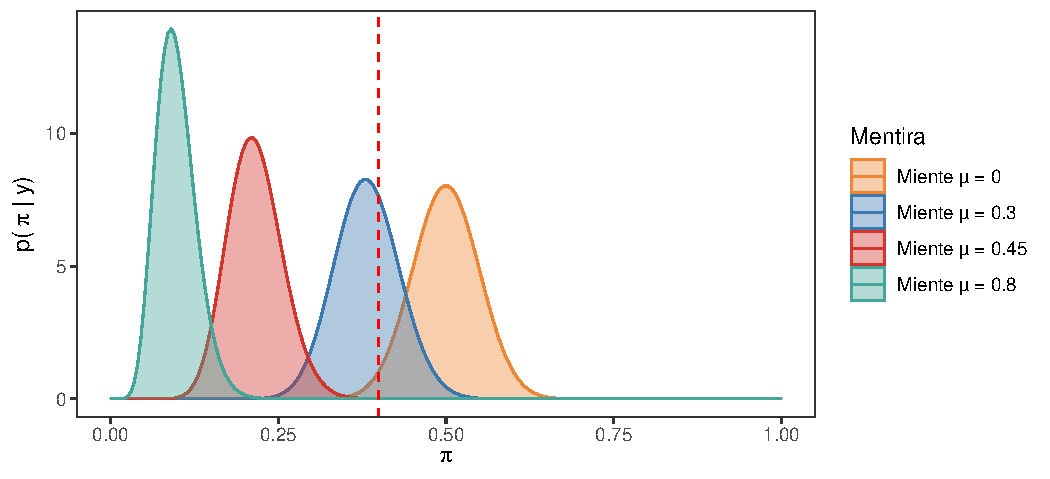
\includegraphics{TP-1--Bayes_files/figure-latex/fig6-1} 

}

\caption{Posterior para los niveles de μ}\label{fig:fig6}
\end{figure}

\begin{figure}

{\centering 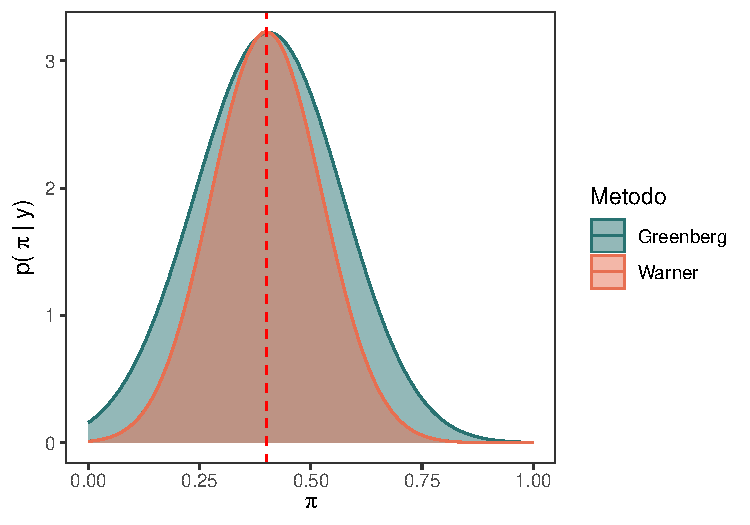
\includegraphics{TP-1--Bayes_files/figure-latex/fig7-1} 

}

\caption{Posterior Greenberg y Warner}\label{fig:fig7}
\end{figure}

\newpage

Para una única muestra proveniente de una población con \(\pi_a=0.4\), se compararon diferentes situaciones, los niveles de mentira \(\mu=0\), \(\mu=0.3\), \(\mu=0.45\), \(\mu=0.8\) y los métodos de respuesta aleatorizada Warner y Greenberg; siendo en total seis comparaciones diferentes. A partir del análisis, se observó en la Figura \ref{fig:fig6} que al aumentar los niveles de mentira, la variabilidad de las distribuciones a posteriori disminuye. Sin embargo, dichas distribuciones se encuentran sesgadas respecto al valor verdadero de \(\pi_a\). Respecto a los métodos Warner y Greenberg, sus \(posterior\) según la muestra utilizada tienden a centrarse en el valor verdadero de \(\pi_a\), lo que indicaría una estimación más precisa. Cabe destacar que, aunque ambos métodos muestran resultados consistentes, el método de Greenberg presenta una variabilidad ligeramente mayor en comparación con el de Warner, lo que puede observarse en la Figura \ref{fig:fig7}. Esta diferencia podría atribuirse a la formulación del mecanismo de respuesta: en el método de Greenberg se utiliza una pregunta no relacionada con la variable de interés, mientras que en el método de Warner se formula una negación de la pregunta original, lo cual podría reducir la dispersión en las respuestas.

\subsubsection{Aumentando la cantidad de simulaciones}\label{subtitulo-12}

Dado que el análisis se basa en una única simulación, no es posible obtener conclusiones respecto a las distribuciones a posteriori, por lo que resulta necesario aumentar la cantidad de simulaciones con el fin de mejorar la evaluación de los posterior para cada situación.

\begin{figure}

{\centering 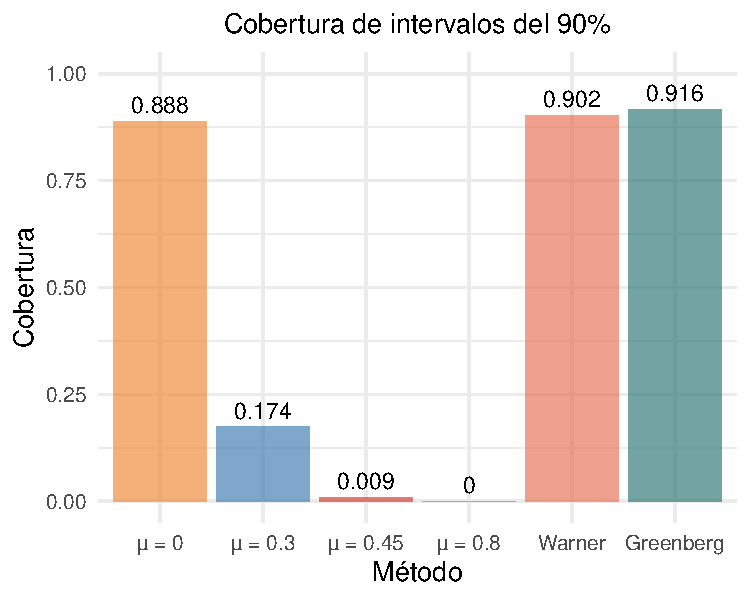
\includegraphics{TP-1--Bayes_files/figure-latex/fig8-1} 

}

\caption{Comparación entre los distintos métodos}\label{fig:fig8}
\end{figure}

Como se observa en la Figura \ref{fig:fig8}, a medida que el nivel de mentira aumenta, la proporción de intervalos de credibilidad del 90\% que incluye al verdadero valor de \(\pi_a\) disminuye de manera considerable. Este fenómeno se evidencia con claridad al comparar el escenario sin mentira, donde la cobertura alcanza aproximadamente un 88.8\%, además en el caso en que el nivel de mentira es \(\mu=0.3\), la cobertura desciende a 17.4\%. Estos resultados permiten concluir, de manera empírica, que considerar el nivel de mentira como parte del modelo resulta fundamental para lograr estimaciones más precisas del valor verdadero de \(\pi_a\).
Por otro lado, se destaca que los métodos de Warner y Greenberg presentan proporciones de cobertura similares, en contraposición a la cobertura observada en la población donde no se miente. Este comportamiento podría atribuirse al supuesto fuerte adoptado en el análisis, según el cual los estudiantes no mienten cuando responden bajo estos métodos.
En resumen, no se observa una gran diferencia entre los métodos considerados, pero sí se observan variaciones importantes en la cobertura según los distintos valores asumidos para el nivel de mentira \(\mu\).

El análisis se centró en la problemática de estudiar la proporción de estudiantes que participan en apuestas en línea, un tema de gran sensibilidad donde la honestidad de las respuestas puede verse comprometida. Se exploraron dos métodos de respuesta aleatorizada, Warner y Greenberg, como estrategias para disminuir el sesgo introducido por la deshonestidad de los estudiantes encuestados. Los resultados obtenidos revelaron que, si bien ambos métodos proporcionan estimaciones más precisas en comparación con los enfoques directos, estos presentan diferencias sutiles en su comportamiento.Específicamente, se observó que el método de Warner tiende a generar distribuciones a posteriori con menor variabilidad, lo que sugiere una incertidumbre menor sobre el estudio del parámetro de interés.
Por otro lado, el análisis de la influencia de los niveles de mentira en las respuestas de los estudiantes demostró que la omisión de este factor en el modelo puede conducir a estimaciones sesgadas y poco confiables. En particular, se evidenció una disminución en la cobertura de los intervalos de credibilidad a medida que aumentaba la probabilidad de que los estudiantes mintieran. En conclusión, este trabajo subraya la importancia de emplear métodos de respuesta aleatorizada al abordar temas sensibles como las apuestas en línea entre adolescentes, y resalta la necesidad de considerar cuidadosamente el efecto que puede tener la cantidad de estudiantes que mienten sobre inferencias.

\end{document}
